\documentclass{standalone}
\usepackage{tikz}
\usetikzlibrary{patterns, positioning}


\begin{document}
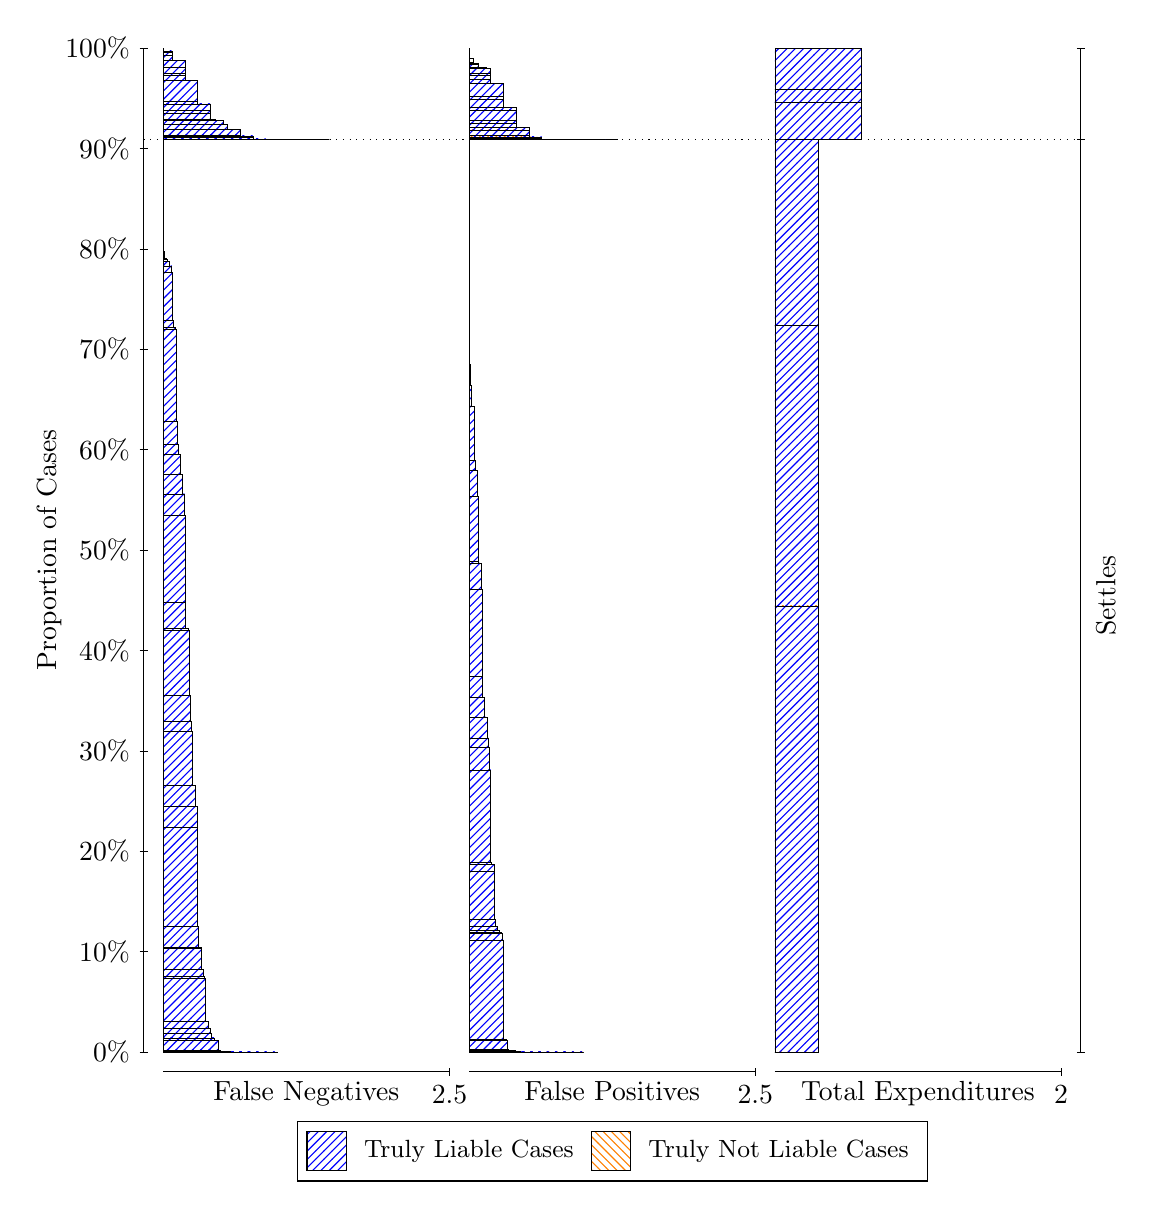
\begin{tikzpicture}
\draw[black, very thin] (1.5,1.75) -- (1.5,14.5);
\node[rotate=90, text=black, anchor=center] at (0.3, 8.125) {Proportion of Cases};
\draw[black, very thin] (1.45,1.75) -- (1.55,1.75);
\node[text=black, anchor=east] at (1.45, 1.75) {0\%};
\draw[black, very thin] (1.45,3.025) -- (1.55,3.025);
\node[text=black, anchor=east] at (1.45, 3.025) {10\%};
\draw[black, very thin] (1.45,4.3) -- (1.55,4.3);
\node[text=black, anchor=east] at (1.45, 4.3) {20\%};
\draw[black, very thin] (1.45,5.575) -- (1.55,5.575);
\node[text=black, anchor=east] at (1.45, 5.575) {30\%};
\draw[black, very thin] (1.45,6.85) -- (1.55,6.85);
\node[text=black, anchor=east] at (1.45, 6.85) {40\%};
\draw[black, very thin] (1.45,8.125) -- (1.55,8.125);
\node[text=black, anchor=east] at (1.45, 8.125) {50\%};
\draw[black, very thin] (1.45,9.4) -- (1.55,9.4);
\node[text=black, anchor=east] at (1.45, 9.4) {60\%};
\draw[black, very thin] (1.45,10.675) -- (1.55,10.675);
\node[text=black, anchor=east] at (1.45, 10.675) {70\%};
\draw[black, very thin] (1.45,11.95) -- (1.55,11.95);
\node[text=black, anchor=east] at (1.45, 11.95) {80\%};
\draw[black, very thin] (1.45,13.225) -- (1.55,13.225);
\node[text=black, anchor=east] at (1.45, 13.225) {90\%};
\draw[black, very thin] (1.45,14.5) -- (1.55,14.5);
\node[text=black, anchor=east] at (1.45, 14.5) {100\%};

\draw[black, very thin] (13.4,1.75) -- (13.4,14.5);
\draw[black, very thin] (13.35,1.75) -- (13.45,1.75);
\node[anchor=west] at (13.35, 1.75) {};
\draw[black, very thin] (13.35,13.337) -- (13.45,13.337);
\node[anchor=west] at (13.35, 13.337) {};
\draw[black, very thin] (13.35,14.5) -- (13.45,14.5);
\node[anchor=west] at (13.35, 14.5) {};

\draw[black, very thin, pattern color=blue, pattern=north east lines] (1.75,1.75) rectangle (3.2033,1.75);
\draw[black, very thin, pattern color=blue, pattern=north east lines] (1.75,1.75) rectangle (3.058,1.75);
\draw[black, very thin, pattern color=blue, pattern=north east lines] (1.75,1.75) rectangle (3.0419,1.75);
\draw[black, very thin, pattern color=blue, pattern=north east lines] (1.75,1.75) rectangle (2.9853,1.75);
\draw[black, very thin, pattern color=blue, pattern=north east lines] (1.75,1.75) rectangle (2.9127,1.75);
\draw[black, very thin, pattern color=blue, pattern=north east lines] (1.75,1.75) rectangle (2.8965,1.75);
\draw[black, very thin, pattern color=blue, pattern=north east lines] (1.75,1.75) rectangle (2.8804,1.75);
\draw[black, very thin, pattern color=blue, pattern=north east lines] (1.75,1.75) rectangle (2.84,1.75);
\draw[black, very thin, pattern color=blue, pattern=north east lines] (1.75,1.75) rectangle (2.8239,1.75);
\draw[black, very thin, pattern color=blue, pattern=north east lines] (1.75,1.75) rectangle (2.7673,1.7501);
\draw[black, very thin, pattern color=blue, pattern=north east lines] (1.75,1.7501) rectangle (2.7512,1.7501);
\draw[black, very thin, pattern color=blue, pattern=north east lines] (1.75,1.7501) rectangle (2.735,1.7501);
\draw[black, very thin, pattern color=blue, pattern=north east lines] (1.75,1.7501) rectangle (2.7189,1.7501);
\draw[black, very thin, pattern color=blue, pattern=north east lines] (1.75,1.7501) rectangle (2.6947,1.7501);
\draw[black, very thin, pattern color=blue, pattern=north east lines] (1.75,1.7501) rectangle (2.6785,1.7501);
\draw[black, very thin, pattern color=blue, pattern=north east lines] (1.75,1.7501) rectangle (2.6624,1.7502);
\draw[black, very thin, pattern color=blue, pattern=north east lines] (1.75,1.7502) rectangle (2.6059,1.7567);
\draw[black, very thin, pattern color=blue, pattern=north east lines] (1.75,1.7567) rectangle (2.5897,1.7567);
\draw[black, very thin, pattern color=blue, pattern=north east lines] (1.75,1.7567) rectangle (2.5736,1.7568);
\draw[black, very thin, pattern color=blue, pattern=north east lines] (1.75,1.7568) rectangle (2.5574,1.7573);
\draw[black, very thin, pattern color=blue, pattern=north east lines] (1.75,1.7573) rectangle (2.5493,1.7573);
\draw[black, very thin, pattern color=blue, pattern=north east lines] (1.75,1.7573) rectangle (2.5332,1.7573);
\draw[black, very thin, pattern color=blue, pattern=north east lines] (1.75,1.7573) rectangle (2.517,1.7597);
\draw[black, very thin, pattern color=blue, pattern=north east lines] (1.75,1.7597) rectangle (2.5009,1.7651);
\draw[black, very thin, pattern color=blue, pattern=north east lines] (1.75,1.7651) rectangle (2.4767,1.7765);
\draw[black, very thin, pattern color=blue, pattern=north east lines] (1.75,1.7765) rectangle (2.4444,1.8968);
\draw[black, very thin, pattern color=blue, pattern=north east lines] (1.75,1.8968) rectangle (2.4282,1.8973);
\draw[black, very thin, pattern color=blue, pattern=north east lines] (1.75,1.8973) rectangle (2.4121,1.9024);
\draw[black, very thin, pattern color=blue, pattern=north east lines] (1.75,1.9024) rectangle (2.3959,1.9287);
\draw[black, very thin, pattern color=blue, pattern=north east lines] (1.75,1.9287) rectangle (2.3879,1.929);
\draw[black, very thin, pattern color=blue, pattern=north east lines] (1.75,1.929) rectangle (2.3717,1.9292);
\draw[black, very thin, pattern color=blue, pattern=north east lines] (1.75,1.9292) rectangle (2.3556,1.9822);
\draw[black, very thin, pattern color=blue, pattern=north east lines] (1.75,1.9822) rectangle (2.3394,2.056);
\draw[black, very thin, pattern color=blue, pattern=north east lines] (1.75,2.056) rectangle (2.3152,2.1404);
\draw[black, very thin, pattern color=blue, pattern=north east lines] (1.75,2.1404) rectangle (2.2829,2.6864);
\draw[black, very thin, pattern color=blue, pattern=north east lines] (1.75,2.6864) rectangle (2.2667,2.7051);
\draw[black, very thin, pattern color=blue, pattern=north east lines] (1.75,2.7051) rectangle (2.2506,2.8002);
\draw[black, very thin, pattern color=blue, pattern=north east lines] (1.75,2.8002) rectangle (2.2344,3.0721);
\draw[black, very thin, pattern color=blue, pattern=north east lines] (1.75,3.0721) rectangle (2.2264,3.0773);
\draw[black, very thin, pattern color=blue, pattern=north east lines] (1.75,3.0773) rectangle (2.2102,3.0798);
\draw[black, very thin, pattern color=blue, pattern=north east lines] (1.75,3.0798) rectangle (2.1941,3.3468);
\draw[black, very thin, pattern color=blue, pattern=north east lines] (1.75,3.3468) rectangle (2.186,4.599);
\draw[black, very thin, pattern color=blue, pattern=north east lines] (1.75,4.599) rectangle (2.1779,4.8686);
\draw[black, very thin, pattern color=blue, pattern=north east lines] (1.75,4.8686) rectangle (2.1537,5.1361);
\draw[black, very thin, pattern color=blue, pattern=north east lines] (1.75,5.1361) rectangle (2.1214,5.8261);
\draw[black, very thin, pattern color=blue, pattern=north east lines] (1.75,5.8261) rectangle (2.1053,5.9441);
\draw[black, very thin, pattern color=blue, pattern=north east lines] (1.75,5.9441) rectangle (2.0891,6.2817);
\draw[black, very thin, pattern color=blue, pattern=north east lines] (1.75,6.2817) rectangle (2.073,7.1018);
\draw[black, very thin, pattern color=blue, pattern=north east lines] (1.75,7.1018) rectangle (2.0649,7.1256);
\draw[black, very thin, pattern color=blue, pattern=north east lines] (1.75,7.1256) rectangle (2.0487,7.1313);
\draw[black, very thin, pattern color=blue, pattern=north east lines] (1.75,7.1313) rectangle (2.0326,7.4659);
\draw[black, very thin, pattern color=blue, pattern=north east lines] (1.75,7.4659) rectangle (2.0245,8.5649);
\draw[black, very thin, pattern color=blue, pattern=north east lines] (1.75,8.5649) rectangle (2.0164,8.8367);
\draw[black, very thin, pattern color=blue, pattern=north east lines] (1.75,8.8367) rectangle (1.9922,9.0824);
\draw[black, very thin, pattern color=blue, pattern=north east lines] (1.75,9.0824) rectangle (1.9599,9.3465);
\draw[black, very thin, pattern color=blue, pattern=north east lines] (1.75,9.3465) rectangle (1.9438,9.4646);
\draw[black, very thin, pattern color=blue, pattern=north east lines] (1.75,9.4646) rectangle (1.9276,9.7539);
\draw[black, very thin, pattern color=blue, pattern=north east lines] (1.75,9.7539) rectangle (1.9115,10.93);
\draw[black, very thin, pattern color=blue, pattern=north east lines] (1.75,10.93) rectangle (1.9034,10.95);
\draw[black, very thin, pattern color=blue, pattern=north east lines] (1.75,10.95) rectangle (1.8873,10.953);
\draw[black, very thin, pattern color=blue, pattern=north east lines] (1.75,10.953) rectangle (1.8711,11.048);
\draw[black, very thin, pattern color=blue, pattern=north east lines] (1.75,11.048) rectangle (1.863,11.654);
\draw[black, very thin, pattern color=blue, pattern=north east lines] (1.75,11.654) rectangle (1.855,11.734);
\draw[black, very thin, pattern color=blue, pattern=north east lines] (1.75,11.734) rectangle (1.8307,11.787);
\draw[black, very thin, pattern color=blue, pattern=north east lines] (1.75,11.787) rectangle (1.7984,11.813);
\draw[black, very thin, pattern color=blue, pattern=north east lines] (1.75,11.813) rectangle (1.7823,11.832);
\draw[black, very thin, pattern color=blue, pattern=north east lines] (1.75,11.832) rectangle (1.7661,11.915);
\draw[black, very thin, pattern color=orange, pattern=north west lines] (1.75,11.915) rectangle (1.75,11.915);
\draw[black, very thin, pattern color=blue, pattern=north east lines] (1.75,11.915) rectangle (1.75,13.337);
\draw[black, very thin, pattern color=blue, pattern=north east lines] (1.75,13.337) rectangle (3.8573,13.337);
\draw[black, very thin, pattern color=blue, pattern=north east lines] (1.75,13.337) rectangle (3.6959,13.337);
\draw[black, very thin, pattern color=blue, pattern=north east lines] (1.75,13.337) rectangle (3.5344,13.337);
\draw[black, very thin, pattern color=blue, pattern=north east lines] (1.75,13.337) rectangle (3.5344,13.337);
\draw[black, very thin, pattern color=blue, pattern=north east lines] (1.75,13.337) rectangle (3.3729,13.337);
\draw[black, very thin, pattern color=blue, pattern=north east lines] (1.75,13.337) rectangle (3.3164,13.337);
\draw[black, very thin, pattern color=blue, pattern=north east lines] (1.75,13.337) rectangle (3.2114,13.338);
\draw[black, very thin, pattern color=blue, pattern=north east lines] (1.75,13.338) rectangle (3.1549,13.338);
\draw[black, very thin, pattern color=blue, pattern=north east lines] (1.75,13.338) rectangle (3.1549,13.338);
\draw[black, very thin, pattern color=blue, pattern=north east lines] (1.75,13.338) rectangle (3.0499,13.346);
\draw[black, very thin, pattern color=blue, pattern=north east lines] (1.75,13.346) rectangle (2.9934,13.346);
\draw[black, very thin, pattern color=blue, pattern=north east lines] (1.75,13.346) rectangle (2.9934,13.346);
\draw[black, very thin, pattern color=blue, pattern=north east lines] (1.75,13.346) rectangle (2.8884,13.362);
\draw[black, very thin, pattern color=blue, pattern=north east lines] (1.75,13.362) rectangle (2.8884,13.384);
\draw[black, very thin, pattern color=blue, pattern=north east lines] (1.75,13.384) rectangle (2.8319,13.384);
\draw[black, very thin, pattern color=blue, pattern=north east lines] (1.75,13.384) rectangle (2.727,13.398);
\draw[black, very thin, pattern color=blue, pattern=north east lines] (1.75,13.398) rectangle (2.727,13.464);
\draw[black, very thin, pattern color=blue, pattern=north east lines] (1.75,13.464) rectangle (2.6704,13.469);
\draw[black, very thin, pattern color=blue, pattern=north east lines] (1.75,13.469) rectangle (2.5655,13.528);
\draw[black, very thin, pattern color=blue, pattern=north east lines] (1.75,13.528) rectangle (2.509,13.529);
\draw[black, very thin, pattern color=blue, pattern=north east lines] (1.75,13.529) rectangle (2.509,13.581);
\draw[black, very thin, pattern color=blue, pattern=north east lines] (1.75,13.581) rectangle (2.404,13.594);
\draw[black, very thin, pattern color=blue, pattern=north east lines] (1.75,13.594) rectangle (2.3475,13.598);
\draw[black, very thin, pattern color=blue, pattern=north east lines] (1.75,13.598) rectangle (2.3475,13.672);
\draw[black, very thin, pattern color=blue, pattern=north east lines] (1.75,13.672) rectangle (2.3475,13.71);
\draw[black, very thin, pattern color=blue, pattern=north east lines] (1.75,13.71) rectangle (2.3475,13.79);
\draw[black, very thin, pattern color=blue, pattern=north east lines] (1.75,13.79) rectangle (2.2425,13.791);
\draw[black, very thin, pattern color=blue, pattern=north east lines] (1.75,13.791) rectangle (2.186,13.822);
\draw[black, very thin, pattern color=blue, pattern=north east lines] (1.75,13.822) rectangle (2.186,14.093);
\draw[black, very thin, pattern color=blue, pattern=north east lines] (1.75,14.093) rectangle (2.081,14.093);
\draw[black, very thin, pattern color=blue, pattern=north east lines] (1.75,14.093) rectangle (2.0245,14.154);
\draw[black, very thin, pattern color=blue, pattern=north east lines] (1.75,14.154) rectangle (2.0245,14.182);
\draw[black, very thin, pattern color=blue, pattern=north east lines] (1.75,14.182) rectangle (2.0245,14.251);
\draw[black, very thin, pattern color=blue, pattern=north east lines] (1.75,14.251) rectangle (2.0245,14.344);
\draw[black, very thin, pattern color=blue, pattern=north east lines] (1.75,14.344) rectangle (1.9196,14.344);
\draw[black, very thin, pattern color=blue, pattern=north east lines] (1.75,14.344) rectangle (1.863,14.406);
\draw[black, very thin, pattern color=blue, pattern=north east lines] (1.75,14.406) rectangle (1.863,14.447);
\draw[black, very thin, pattern color=blue, pattern=north east lines] (1.75,14.447) rectangle (1.863,14.465);
\draw[black, very thin, pattern color=blue, pattern=north east lines] (1.75,14.465) rectangle (1.7581,14.465);
\draw[black, very thin, pattern color=orange, pattern=north west lines] (1.75,14.465) rectangle (1.75,14.465);
\draw[black, very thin, pattern color=blue, pattern=north east lines] (1.75,14.465) rectangle (1.75,14.5);
\draw[black, very thin, pattern color=orange, pattern=north west lines] (5.6333,1.75) rectangle (7.0867,1.75);
\draw[black, very thin, pattern color=blue, pattern=north east lines] (5.6333,1.75) rectangle (7.0867,1.75);
\draw[black, very thin, pattern color=blue, pattern=north east lines] (5.6333,1.75) rectangle (6.9252,1.75);
\draw[black, very thin, pattern color=orange, pattern=north west lines] (5.6333,1.75) rectangle (6.796,1.75);
\draw[black, very thin, pattern color=blue, pattern=north east lines] (5.6333,1.75) rectangle (6.796,1.75);
\draw[black, very thin, pattern color=blue, pattern=north east lines] (5.6333,1.75) rectangle (6.7637,1.75);
\draw[black, very thin, pattern color=orange, pattern=north west lines] (5.6333,1.75) rectangle (6.7233,1.75);
\draw[black, very thin, pattern color=blue, pattern=north east lines] (5.6333,1.75) rectangle (6.7233,1.75);
\draw[black, very thin, pattern color=blue, pattern=north east lines] (5.6333,1.75) rectangle (6.6345,1.75);
\draw[black, very thin, pattern color=blue, pattern=north east lines] (5.6333,1.75) rectangle (6.6022,1.75);
\draw[black, very thin, pattern color=orange, pattern=north west lines] (5.6333,1.75) rectangle (6.578,1.75);
\draw[black, very thin, pattern color=blue, pattern=north east lines] (5.6333,1.75) rectangle (6.578,1.75);
\draw[black, very thin, pattern color=blue, pattern=north east lines] (5.6333,1.75) rectangle (6.5619,1.75);
\draw[black, very thin, pattern color=orange, pattern=north west lines] (5.6333,1.75) rectangle (6.5053,1.75);
\draw[black, very thin, pattern color=blue, pattern=north east lines] (5.6333,1.75) rectangle (6.5053,1.75);
\draw[black, very thin, pattern color=blue, pattern=north east lines] (5.6333,1.75) rectangle (6.473,1.75);
\draw[black, very thin, pattern color=blue, pattern=north east lines] (5.6333,1.75) rectangle (6.4407,1.75);
\draw[black, very thin, pattern color=orange, pattern=north west lines] (5.6333,1.75) rectangle (6.4327,1.75);
\draw[black, very thin, pattern color=blue, pattern=north east lines] (5.6333,1.75) rectangle (6.4327,1.75);
\draw[black, very thin, pattern color=blue, pattern=north east lines] (5.6333,1.75) rectangle (6.4165,1.75);
\draw[black, very thin, pattern color=blue, pattern=north east lines] (5.6333,1.75) rectangle (6.4004,1.75);
\draw[black, very thin, pattern color=orange, pattern=north west lines] (5.6333,1.75) rectangle (6.36,1.75);
\draw[black, very thin, pattern color=blue, pattern=north east lines] (5.6333,1.75) rectangle (6.36,1.7501);
\draw[black, very thin, pattern color=blue, pattern=north east lines] (5.6333,1.7501) rectangle (6.3439,1.7501);
\draw[black, very thin, pattern color=blue, pattern=north east lines] (5.6333,1.7501) rectangle (6.3116,1.7501);
\draw[black, very thin, pattern color=orange, pattern=north west lines] (5.6333,1.7501) rectangle (6.2873,1.7501);
\draw[black, very thin, pattern color=blue, pattern=north east lines] (5.6333,1.7501) rectangle (6.2873,1.7505);
\draw[black, very thin, pattern color=blue, pattern=north east lines] (5.6333,1.7505) rectangle (6.2793,1.7562);
\draw[black, very thin, pattern color=blue, pattern=north east lines] (5.6333,1.7562) rectangle (6.2712,1.7562);
\draw[black, very thin, pattern color=blue, pattern=north east lines] (5.6333,1.7562) rectangle (6.255,1.7563);
\draw[black, very thin, pattern color=blue, pattern=north east lines] (5.6333,1.7563) rectangle (6.2389,1.7563);
\draw[black, very thin, pattern color=orange, pattern=north west lines] (5.6333,1.7563) rectangle (6.2147,1.7563);
\draw[black, very thin, pattern color=blue, pattern=north east lines] (5.6333,1.7563) rectangle (6.2147,1.7673);
\draw[black, very thin, pattern color=blue, pattern=north east lines] (5.6333,1.7673) rectangle (6.1985,1.7679);
\draw[black, very thin, pattern color=blue, pattern=north east lines] (5.6333,1.7679) rectangle (6.1824,1.7684);
\draw[black, very thin, pattern color=blue, pattern=north east lines] (5.6333,1.7684) rectangle (6.1501,1.7708);
\draw[black, very thin, pattern color=blue, pattern=north east lines] (5.6333,1.7708) rectangle (6.1259,1.7792);
\draw[black, very thin, pattern color=blue, pattern=north east lines] (5.6333,1.7792) rectangle (6.1178,1.9005);
\draw[black, very thin, pattern color=blue, pattern=north east lines] (5.6333,1.9005) rectangle (6.1097,1.9057);
\draw[black, very thin, pattern color=blue, pattern=north east lines] (5.6333,1.9057) rectangle (6.0936,1.9059);
\draw[black, very thin, pattern color=blue, pattern=north east lines] (5.6333,1.9059) rectangle (6.0774,1.9089);
\draw[black, very thin, pattern color=orange, pattern=north west lines] (5.6333,1.9089) rectangle (6.0693,1.9089);
\draw[black, very thin, pattern color=blue, pattern=north east lines] (5.6333,1.9089) rectangle (6.0693,3.1721);
\draw[black, very thin, pattern color=blue, pattern=north east lines] (5.6333,3.1721) rectangle (6.0532,3.2543);
\draw[black, very thin, pattern color=blue, pattern=north east lines] (5.6333,3.2543) rectangle (6.037,3.2732);
\draw[black, very thin, pattern color=blue, pattern=north east lines] (5.6333,3.2732) rectangle (6.0209,3.2994);
\draw[black, very thin, pattern color=blue, pattern=north east lines] (5.6333,3.2994) rectangle (5.9886,3.3526);
\draw[black, very thin, pattern color=blue, pattern=north east lines] (5.6333,3.3526) rectangle (5.9644,3.4325);
\draw[black, very thin, pattern color=blue, pattern=north east lines] (5.6333,3.4325) rectangle (5.9563,4.0388);
\draw[black, very thin, pattern color=blue, pattern=north east lines] (5.6333,4.0388) rectangle (5.9482,4.1338);
\draw[black, very thin, pattern color=blue, pattern=north east lines] (5.6333,4.1338) rectangle (5.9321,4.1363);
\draw[black, very thin, pattern color=blue, pattern=north east lines] (5.6333,4.1363) rectangle (5.9159,4.1569);
\draw[black, very thin, pattern color=blue, pattern=north east lines] (5.6333,4.1569) rectangle (5.9079,5.3327);
\draw[black, very thin, pattern color=blue, pattern=north east lines] (5.6333,5.3327) rectangle (5.8917,5.622);
\draw[black, very thin, pattern color=blue, pattern=north east lines] (5.6333,5.622) rectangle (5.8756,5.7401);
\draw[black, very thin, pattern color=blue, pattern=north east lines] (5.6333,5.7401) rectangle (5.8594,6.0042);
\draw[black, very thin, pattern color=blue, pattern=north east lines] (5.6333,6.0042) rectangle (5.8271,6.2499);
\draw[black, very thin, pattern color=blue, pattern=north east lines] (5.6333,6.2499) rectangle (5.8029,6.5217);
\draw[black, very thin, pattern color=blue, pattern=north east lines] (5.6333,6.5217) rectangle (5.7948,7.6207);
\draw[black, very thin, pattern color=blue, pattern=north east lines] (5.6333,7.6207) rectangle (5.7867,7.9553);
\draw[black, very thin, pattern color=blue, pattern=north east lines] (5.6333,7.9553) rectangle (5.7706,7.961);
\draw[black, very thin, pattern color=blue, pattern=north east lines] (5.6333,7.961) rectangle (5.7544,7.9848);
\draw[black, very thin, pattern color=blue, pattern=north east lines] (5.6333,7.9848) rectangle (5.7464,8.8048);
\draw[black, very thin, pattern color=blue, pattern=north east lines] (5.6333,8.8048) rectangle (5.7302,9.1425);
\draw[black, very thin, pattern color=blue, pattern=north east lines] (5.6333,9.1425) rectangle (5.7141,9.2605);
\draw[black, very thin, pattern color=blue, pattern=north east lines] (5.6333,9.2605) rectangle (5.6979,9.9505);
\draw[black, very thin, pattern color=blue, pattern=north east lines] (5.6333,9.9505) rectangle (5.6656,10.218);
\draw[black, very thin, pattern color=blue, pattern=north east lines] (5.6333,10.218) rectangle (5.6414,10.488);
\draw[black, very thin, pattern color=blue, pattern=north east lines] (5.6333,10.488) rectangle (5.6333,13.337);
\draw[black, very thin, pattern color=orange, pattern=north west lines] (5.6333,13.337) rectangle (7.5227,13.337);
\draw[black, very thin, pattern color=blue, pattern=north east lines] (5.6333,13.337) rectangle (7.5227,13.337);
\draw[black, very thin, pattern color=orange, pattern=north west lines] (5.6333,13.337) rectangle (7.3612,13.337);
\draw[black, very thin, pattern color=blue, pattern=north east lines] (5.6333,13.337) rectangle (7.3612,13.337);
\draw[black, very thin, pattern color=blue, pattern=north east lines] (5.6333,13.337) rectangle (7.1997,13.337);
\draw[black, very thin, pattern color=orange, pattern=north west lines] (5.6333,13.337) rectangle (7.1997,13.337);
\draw[black, very thin, pattern color=blue, pattern=north east lines] (5.6333,13.337) rectangle (7.1997,13.337);
\draw[black, very thin, pattern color=blue, pattern=north east lines] (5.6333,13.337) rectangle (7.0382,13.337);
\draw[black, very thin, pattern color=blue, pattern=north east lines] (5.6333,13.337) rectangle (7.0382,13.337);
\draw[black, very thin, pattern color=orange, pattern=north west lines] (5.6333,13.337) rectangle (7.0382,13.337);
\draw[black, very thin, pattern color=blue, pattern=north east lines] (5.6333,13.337) rectangle (7.0382,13.337);
\draw[black, very thin, pattern color=orange, pattern=north west lines] (5.6333,13.337) rectangle (6.8767,13.337);
\draw[black, very thin, pattern color=blue, pattern=north east lines] (5.6333,13.337) rectangle (6.8767,13.337);
\draw[black, very thin, pattern color=blue, pattern=north east lines] (5.6333,13.337) rectangle (6.8767,13.337);
\draw[black, very thin, pattern color=blue, pattern=north east lines] (5.6333,13.337) rectangle (6.8767,13.337);
\draw[black, very thin, pattern color=orange, pattern=north west lines] (5.6333,13.337) rectangle (6.7153,13.337);
\draw[black, very thin, pattern color=blue, pattern=north east lines] (5.6333,13.337) rectangle (6.7153,13.341);
\draw[black, very thin, pattern color=blue, pattern=north east lines] (5.6333,13.341) rectangle (6.7153,13.342);
\draw[black, very thin, pattern color=blue, pattern=north east lines] (5.6333,13.342) rectangle (6.5538,13.355);
\draw[black, very thin, pattern color=orange, pattern=north west lines] (5.6333,13.355) rectangle (6.5538,13.355);
\draw[black, very thin, pattern color=blue, pattern=north east lines] (5.6333,13.355) rectangle (6.5538,13.372);
\draw[black, very thin, pattern color=orange, pattern=north west lines] (5.6333,13.372) rectangle (6.4973,13.372);
\draw[black, very thin, pattern color=blue, pattern=north east lines] (5.6333,13.372) rectangle (6.4973,13.372);
\draw[black, very thin, pattern color=blue, pattern=north east lines] (5.6333,13.372) rectangle (6.3923,13.389);
\draw[black, very thin, pattern color=blue, pattern=north east lines] (5.6333,13.389) rectangle (6.3923,13.459);
\draw[black, very thin, pattern color=orange, pattern=north west lines] (5.6333,13.459) rectangle (6.3923,13.459);
\draw[black, very thin, pattern color=blue, pattern=north east lines] (5.6333,13.459) rectangle (6.3923,13.493);
\draw[black, very thin, pattern color=blue, pattern=north east lines] (5.6333,13.493) rectangle (6.3358,13.493);
\draw[black, very thin, pattern color=orange, pattern=north west lines] (5.6333,13.493) rectangle (6.3358,13.493);
\draw[black, very thin, pattern color=blue, pattern=north east lines] (5.6333,13.493) rectangle (6.3358,13.493);
\draw[black, very thin, pattern color=blue, pattern=north east lines] (5.6333,13.493) rectangle (6.2308,13.548);
\draw[black, very thin, pattern color=blue, pattern=north east lines] (5.6333,13.548) rectangle (6.2308,13.581);
\draw[black, very thin, pattern color=blue, pattern=north east lines] (5.6333,13.581) rectangle (6.2308,13.713);
\draw[black, very thin, pattern color=blue, pattern=north east lines] (5.6333,13.713) rectangle (6.2308,13.715);
\draw[black, very thin, pattern color=blue, pattern=north east lines] (5.6333,13.715) rectangle (6.2308,13.743);
\draw[black, very thin, pattern color=orange, pattern=north west lines] (5.6333,13.743) rectangle (6.1743,13.743);
\draw[black, very thin, pattern color=blue, pattern=north east lines] (5.6333,13.743) rectangle (6.1743,13.743);
\draw[black, very thin, pattern color=blue, pattern=north east lines] (5.6333,13.743) rectangle (6.1743,13.743);
\draw[black, very thin, pattern color=blue, pattern=north east lines] (5.6333,13.743) rectangle (6.0693,13.85);
\draw[black, very thin, pattern color=blue, pattern=north east lines] (5.6333,13.85) rectangle (6.0693,13.882);
\draw[black, very thin, pattern color=blue, pattern=north east lines] (5.6333,13.882) rectangle (6.0693,14.046);
\draw[black, very thin, pattern color=blue, pattern=north east lines] (5.6333,14.046) rectangle (6.0128,14.046);
\draw[black, very thin, pattern color=orange, pattern=north west lines] (5.6333,14.046) rectangle (6.0128,14.046);
\draw[black, very thin, pattern color=blue, pattern=north east lines] (5.6333,14.046) rectangle (6.0128,14.047);
\draw[black, very thin, pattern color=blue, pattern=north east lines] (5.6333,14.047) rectangle (5.9079,14.106);
\draw[black, very thin, pattern color=blue, pattern=north east lines] (5.6333,14.106) rectangle (5.9079,14.156);
\draw[black, very thin, pattern color=blue, pattern=north east lines] (5.6333,14.156) rectangle (5.9079,14.182);
\draw[black, very thin, pattern color=blue, pattern=north east lines] (5.6333,14.182) rectangle (5.9079,14.242);
\draw[black, very thin, pattern color=blue, pattern=north east lines] (5.6333,14.242) rectangle (5.8513,14.244);
\draw[black, very thin, pattern color=orange, pattern=north west lines] (5.6333,14.244) rectangle (5.8513,14.244);
\draw[black, very thin, pattern color=blue, pattern=north east lines] (5.6333,14.244) rectangle (5.8513,14.244);
\draw[black, very thin, pattern color=blue, pattern=north east lines] (5.6333,14.244) rectangle (5.8513,14.255);
\draw[black, very thin, pattern color=blue, pattern=north east lines] (5.6333,14.255) rectangle (5.7464,14.288);
\draw[black, very thin, pattern color=blue, pattern=north east lines] (5.6333,14.288) rectangle (5.7464,14.308);
\draw[black, very thin, pattern color=blue, pattern=north east lines] (5.6333,14.308) rectangle (5.6899,14.315);
\draw[black, very thin, pattern color=blue, pattern=north east lines] (5.6333,14.315) rectangle (5.6899,14.317);
\draw[black, very thin, pattern color=blue, pattern=north east lines] (5.6333,14.317) rectangle (5.6899,14.368);
\draw[black, very thin, pattern color=blue, pattern=north east lines] (5.6333,14.368) rectangle (5.6333,14.5);
\draw[black, very thin, pattern color=orange, pattern=north west lines] (9.5167,1.75) rectangle (10.062,1.75);
\draw[black, very thin, pattern color=blue, pattern=north east lines] (9.5167,1.75) rectangle (10.062,7.4155);
\draw[black, very thin, pattern color=orange, pattern=north west lines] (9.5167,7.4155) rectangle (10.062,7.4155);
\draw[black, very thin, pattern color=blue, pattern=north east lines] (9.5167,7.4155) rectangle (10.062,10.973);
\draw[black, very thin, pattern color=orange, pattern=north west lines] (9.5167,10.973) rectangle (10.062,10.973);
\draw[black, very thin, pattern color=blue, pattern=north east lines] (9.5167,10.973) rectangle (10.062,13.337);
\draw[black, very thin, pattern color=orange, pattern=north west lines] (9.5167,13.337) rectangle (10.607,13.337);
\draw[black, very thin, pattern color=blue, pattern=north east lines] (9.5167,13.337) rectangle (10.607,13.812);
\draw[black, very thin, pattern color=orange, pattern=north west lines] (9.5167,13.812) rectangle (10.607,13.812);
\draw[black, very thin, pattern color=blue, pattern=north east lines] (9.5167,13.812) rectangle (10.607,13.973);
\draw[black, very thin, pattern color=orange, pattern=north west lines] (9.5167,13.973) rectangle (10.607,13.973);
\draw[black, very thin, pattern color=blue, pattern=north east lines] (9.5167,13.973) rectangle (10.607,14.5);
\draw[black, dotted] (1.5,13.337) -- (13.4,13.337);
\draw[black, very thin] (1.75,1.5) -- (5.3833,1.5);
\node[text=black, anchor=north] at (3.5667, 1.5) {False Negatives};
\draw[black, very thin] (5.3833,1.45) -- (5.3833,1.55);
\node[text=black, anchor=north] at (5.3833, 1.45) {2.5};

\draw[black, very thin] (5.6333,1.5) -- (9.2667,1.5);
\node[text=black, anchor=north] at (7.45, 1.5) {False Positives};
\draw[black, very thin] (9.2667,1.45) -- (9.2667,1.55);
\node[text=black, anchor=north] at (9.2667, 1.45) {2.5};

\draw[black, very thin] (9.5167,1.5) -- (13.15,1.5);
\node[text=black, anchor=north] at (11.333, 1.5) {Total Expenditures};
\draw[black, very thin] (13.15,1.45) -- (13.15,1.55);
\node[text=black, anchor=north] at (13.15, 1.45) {2};

\node[text=black, centered, rotate=90] at (13.72, 7.5433) {Settles};


\draw (7.449999999999999,1.5) node[draw=none] (baseCoordinate) {};
\begin{scope}[align=center]
        \matrix[scale=0.5, draw=black, below=0.5cm of baseCoordinate, nodes={draw}, column sep=0.1cm]{
            \node[rectangle, draw, minimum width=0.5cm, minimum height=0.5cm, pattern color=blue, pattern=north east lines] {}; &
            \node[draw=none, font=\small, text=black] (B) {Truly Liable Cases}; &
            \node[rectangle, draw, minimum width=0.5cm, minimum height=0.5cm, pattern color=orange, pattern=north west lines] {}; &
            \node[draw=none, font=\small, text=black] (B) {Truly Not Liable Cases}; \\
            };
\end{scope}

\end{tikzpicture}
\end{document}